%Cria um tópico (que pode conter vários slides)
\section[Plataforma]{Plataforma Java}

%Cria um sub-tópico
\subsection{Apresentação}

%Cria um slide para o tópico/sub-tópico atuals
\frame{\frametitle{Plataforma Java - Apresentação}
\begin{itemize}
  \item Multi-linguagem. Tem como principal a linguagem Java
  \item Permite que aplicações desenvolvidas sejam executadas em diferentes hardwares e sistema operacionais 
  \item Necessidade de uma Máquina Virtual Java (Java Virtual Machine - JVM/Java Runtime Environment - JRE) para execução de aplicações
  \item JVM específica para cada hardware e SO
\end{itemize}  
}

%Outro slide
\frame{\frametitle{Plataforma Java - Apresentação}
\begin{itemize}
  \item Bytecodes (.class): interpretados pela JVM. Compilados a partir dos arquivos fonte
  (normalmente arquivos .java)
  \item Just In Time Compiler (JIT): compilação de bytecodes para código de máquina na primeira execução
\end{itemize}
\begin{center}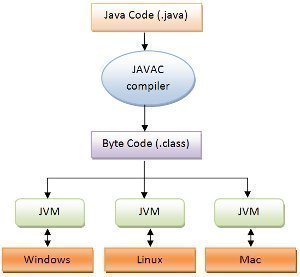
\includegraphics[scale=0.3]{imgs/Java-Bytecode.png}\end{center} 
Imagem: \url{http://www.tech-faq.com/java-bytecode.html}
}

%Cria um sub-sub tópico
\subsubsection{Edições}

%Cria um slide para o tópico anterior
\frame{\frametitle{Plataforma Java - Edições}
\begin{itemize}
  \item Java Standard Edition - JSE (antiga J2SE): plataforma base para o desenvolvimento de aplicações de uso geral em Java, como aplicações console ou desktop.
  \item Java Enterprise Edition - JEE (antiga J2EE): plataforma para o desenvolvimento de aplicações de Web
  \item Java Micro Edition - JME (antiga J2ME): plataforma para o desenvolvimento de aplicações para sistemas embarcadas (como celulares, smartphones e TV's).
  \begin{itemize}
  \item Perdeu mercado p/ novas plataformas (iPhone, Android, Windows Phone ...)
  \end{itemize}
  \item Java Card: plataforma para desenvolvimento de aplicações embarcadas em cartões 
  (como cartões de crédito com chip, SIM Cards, etc) e dispositivos
  extremamente restritos de recursos de hardware.
\end{itemize}
}

%Cria outro sub-sub tópico
\subsubsection{Linguagens}

%Cria um slide para o tópico anterior
\frame{\frametitle{Plataforma Java - Linguagens}
\begin{itemize}
  \item Não restrita ao uso da linguagem Java. Algumas linguagens que podem ser utilizadas:
  \begin{itemize}
  \item Groovy
  \item Ruby (usando JRuby)
  \item Python (usando Jython)
  \item JavaScript (usando Rhino)
  \end{itemize}
\end{itemize}
}
      

%Cria outro sub-sub tópico
\subsubsection[Dev/Exec]{Desenvolvimento e Execução}

%Cria um slide para o tópico anterior
\frame{\frametitle{Plataforma Java - Desenvolvimento e Execução}
\begin{itemize}
  \item Java Development Kit (JDK): contém ferramentas básicas para desenvolvimento de aplicações Java. Alguns itens do JDK:
  \begin{itemize}
  \item javac – Compilador bytecode
  \item java – Interpretador de bytecodes (.class)
  \item javadoc – Geração de documentação (em HTML) de aplicações Java
  \item jar – Empacotador de aplicações Java
  \item javap – Descompilador de arquivos .class
  \item javaws – Java Web Start para execução de aplicações JNLP
  \end{itemize}
  \item Java Runtime Environment (JRE): contém a JVM para execução de aplicações desenvolvidas para a plataforma Java  
\end{itemize}
}

%Cria outro slide para o tópico anterior
\frame{\frametitle{Plataforma Java - Desenvolvimento e Execução}
\begin{itemize}
  \item Devido às suas especificações livres, surgiram implementações
da comunidade:
  \begin{itemize}
  \item Open JDK / Open JRE
  \item GNU Compiler for Java: GCJ
  \end{itemize}
\end{itemize}
}
